\documentclass[oneside,fontset=founder]{ctexbook}

\usepackage{geometry}% 用于页面设置
\usepackage[dvipsnames, svgnames, x11names]{xcolor}% 颜色支持
\usepackage{graphicx}% 图形支持
\usepackage[
  colorlinks=true,
  linkcolor=Navy,
  urlcolor=Navy,
  citecolor=Navy,
  anchorcolor=Navy
]{hyperref}% 设置超链接颜色
\usepackage{enumerate}% 枚举支持
\usepackage{minted}% 代码显示支持

% 纸张设置
\geometry{
  b5paper,
  left = 1in,
  right = 1in,
  top = 1in,
  bottom = 1in
}

% 设置章节标题左对齐,+=表示在原有格式上追加,如果只有=则表示完全替换
\ctexset{
  chapter/format += \raggedright,
  section/format += \raggedright,
  subsection/format += \raggedright,
  subsubsection/format += \raggedright,
}

\emergencystretch = \maxdimen% 断字处理
\setlength{\parindent}{2em}% 缩进
\setlength{\parskip}{1ex} % 段间距

% 定义颜色
% \definecolor{pageYellow}{HTML}{F2F1D7}

% \pagecolor{pageYellow}


% ------------------ 开始 -------------------


\begin{document}


% ------------------ 封面 -------------------
\begin{titlepage}%
\begin{center}
  \quad

  \vspace{2ex}

  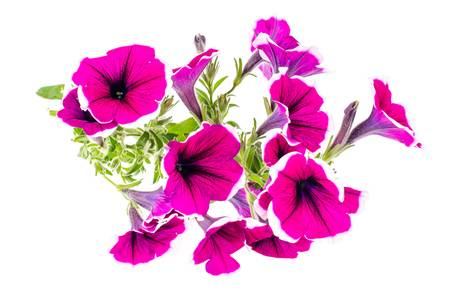
\includegraphics[width=.4\textwidth]{images/cover.png}

  \vspace{4ex}

  \Huge\heiti Petunia项目开发记录\normalsize\normalfont

  \vspace{4ex}

  陆巍
  \vfill%
  % Bottom of the page
  2023年10月5日
\end{center}
\end{titlepage}


% ------------------ 前言 -------------------
\frontmatter% 关闭章节序号,页码使用罗马数字


\chapter{前言}



% ------------------ 目录 -------------------
\tableofcontents% 生成目录


% ------------------ 正文 -------------------
\mainmatter


\chapter{开发日记}


\section{2023年10月}


\subsection{10月5日}
这个项目最初只是打算使用简单的判断方法来解决,但想到以后要开发其他编译器,所以先用这个微小项目来练练手。项目将按照编译器开发方法来实现,当然,本项目过于微小,大概只会用到词法分析与语法分析。

Windows系统和Linux系统在文本处理上是有些差异的,其中的换行就不相同。Windows系统中的换行实际上包含了两个字符,即$\backslash r$(回车,0xD)与$\backslash n$(换行,0xA),而Linux系统中只有$\backslash n$(换行,0xA)。我现在主要使用的是Linux系统,但为了兼顾Windows系统,可能需要在读入配置文件后,先把其中的$\backslash r\backslash n$替换成$\backslash n$,然后才做词法分析。
\end{document}